\chapter{Esperimenti}\label{ch:chapter2}

Per la valutazione delle metriche sono stati condotti diversi esperimenti che possono essere suddivisi in due macro-categorie dipendentemente dal tipo di dataset utilizzato:
\begin{itemize}
    \item \textbf{Toy Dataset}: dataset generati artificialmente per testare il comportamento delle metriche in condizioni controllate.
    \item \textbf{Real World Dataset}: dataset reali per testare il comportamento delle metriche in condizioni reali.
\end{itemize}
Le sezioni seguenti descrivono come sono state implementate le metriche, gli esperimenti così come le distribuzioni di dati utilizzate.\
La ragione per cui sono stati condotti esperimenti su dateset generati artificilmente (ovvero di matrice matematica, non derivanti dalla realtà o generati da reti neurali) è che in questo modo è stato possibile osservare il comportamento delle metriche in condizioni controllate, ideali e per poter confrontare i risultati ottenuti con quelli attesi presenti nella letteratura.\
Fanno infatti parte dei test su 'toy dataset', i test di corretta implementazione ovvero un'analisi comparativa delle diverse implementazioni in codice delle metriche. Tali test hanno il fine di verificare che le metriche restituiscano valori corretti validando gli altri esperimenti.\

I dataset reali sono stati utilizzati per testare il comportamento delle metriche in condizioni reali, ovvero per verificare se le metriche si comportano come ci si aspetta in situazioni non ben definite, con distribuzioni di dati non note, ben distanti da quelle ideali. Questo infatti, come vedremo, può sollevare criticità, ad esempio dovute alla assenza di certe categorie di dati o alla presenza di dati non ben distribuiti.\
Un altro elemento dei dataset reali è che spesso questi non sono di carattere prettamente numerico, nei dataset analizzati ad esempio, abbiamo immagini di farfalle e partiture musicali. Questo comporta la necessità di trasformare i dati per poterli utilizzare, e il processo di \textbf{estrazioni di caratteristiche} può equivalere ad una perdita di dati significativi o, al contrario, ad una sovrabbondanza di dati non significativi.\

\section{Toy Dataset}
\label{sec:toy-dataset}

Come anticipato nell’introduzione di questo capitolo, i Toy Dataset sono dataset generati artificialmente tramite funzioni matematiche che producono dati in modo casuale ma controllato. Per questi esperimenti, sono state utilizzate principalmente due tipi di distribuzioni di dati numerici con dimensione variabile: la distribuzione uniforme e la distribuzione normale. In una specifica categoria di esperimenti, sono stati aggiunti anche outliers, ossia dati che si discostano significativamente dalla distribuzione principale, con l'obiettivo di valutare la robustezza delle metriche in presenza di anomalie.

Gli esperimenti condotti si ispirano a quelli presenti in letteratura e hanno diversi obiettivi, tra cui:
\begin{itemize}
    \item Testare l'influenza degli iperparametri delle metriche sul loro comportamento.
    \item Valutare la risposta delle metriche alla presenza di outliers.
    \item Studiare l'impatto della dimensione del dataset sui risultati.
    \item Confrontare le implementazioni delle metriche esistenti comparando numericamente i risultati su dataset identici e confrontando i grafici delle pr-curve con quelli presenti in letteratura.
\end{itemize}

Per ciascun esperimento sono stati prodotti grafici che illustrano i risultati ottenuti. L'unica eccezione è rappresentata dai test di corretta implementazione delle metriche, dove la validazione è stata condotta principalmente tramite confronti numerici. La scelta delle tipologie di grafici è stata guidata dall'obiettivo di facilitare il confronto con i risultati riportati in letteratura quindi in certe circostanza anche a discapito della chiarezza dei grafici stessi.

Data la complessità computazionale di alcuni esperimenti, i risultati intermedi e finali sono stati salvati in file \texttt{.npy}, permettendo analisi approfondite e riproducibilità senza dover ripetere calcoli onerosi. Questo approccio non solo consente una gestione efficiente dei dati, ma permette anche un'analisi successiva più flessibile, ad esempio per esplorare ulteriori correlazioni, per verificare ipotesi aggiuntive o per produrre grafici alternativi.

\subsection{Parametro k e dimensione del dataset}
\label{subsec:k-dataset-dimension}

Come abbiamo visto, tutte le metriche analizzate si basano sulla distanza dei dati rispetto ai loro vicini. Uno dei parametri più determinanti è l'ordine \texttt{k} del vicino più prossimo. Secondo la letteratura, i valori ottimali di \texttt{k} variano in base alla metrica analizzata: per l’\textbf{improved precision recall} \texttt{k = 3}, per la \textbf{probabilistic precision recall} \texttt{k = 4}, per la \textbf{precision recall coverage} \texttt{k=\(\sqrt{|\Phi|}\)} indicando con \(|\Phi|\) la dimensione del dataset reale e/o generato (o \texttt{k = 3} se \texttt{C = 3})
, mentre per \textbf{density} e \textbf{coverage} \texttt{k = 5}. Questi valori riflettono un compromesso ottimale tra stabilità della metrica e sensibilità alla densità locale. Ci si aspetta che l'aumento della dimensione del dataset porti a un incremento dei valori delle metriche, poiché una maggiore quantità di dati aumenta la densità dei punti, migliorando la rappresentatività delle distribuzioni e riducendo l’effetto del rumore.

L'analisi è stata condotta su dataset generati una sola volta, mantenuti costanti e identici per la valutazione di tutte le metriche, questo per garantire coerenza nei risultati. Sono state utilizzate, come anticipato precedentemente, due diverse distribuzioni: uniforme e normale. I test sono stati effettuati per valori di \texttt{k} variabili da 1 a 10 vale a dire \([1,2,3,\dots,8,9,10]\) e per dimensioni del dataset crescenti esponenzialmente, da 500 a 16000 punti (\([500,1000,2000,4000,8000,16000]\)). Ogni dato è rappresentato come un vettore in \(\mathbb{R}^{64}\).

Per presentare i risultati, sono state utilizzate delle \textbf{heatmap}, che mostrano i valori delle metriche in funzione di \texttt{k} e della dimensione del dataset. In queste rappresentazioni, il rosso indica valori prossimi a \texttt{1.}, mentre il verde valori vicini a \texttt{0.}. Sebbene le heatmap non offrano precisione numerica immediata, forniscono una visione d’insieme sulle tendenze generali delle metriche e facilitano il confronto con gli esperimenti presenti in letteratura \cite{3ReliableFidelityDiversityMetrics}. Nel paper di riferimento, sono state prodotte heatmap solo per le metriche di \textbf{improved precision recall} e \textbf{density and coverage} e con distribuzioni normali identiche, ma per completezza sono state prodotte anche per le altre metriche presentate nel capitolo precedente e per distribuzioni uniformi, per evidenziare eventuali comportamenti che si possono presentare in situazioni diverse.

\subsection{Dimensione del dataset e dimensione dei dati}
\label{subsec:dataset-data-dimension}

In questo caso, l'analisi condotta non ha un riscontro diretto nella letteratura esistente, ovvero non presenta antecedenti (quantomeno per gli articoli presi in analisi). L'obiettivo è determinare come la \textbf{dimensione del dataset} possa influenzare la densità dei dati della distribuzione (a dimensione dei dati fissata) e, conseguentemente, il valore delle metriche. I risultati di questa analisi costituiscono una parte fondamentale per le analisi su dati reali, dove la scelta del numero di caratteristiche da considerare può risultare determinante.

In questo esperimento, abbiamo considerato una distribuzione normale (\(\mathcal{N}(0, I)\)) dei dati con \textbf{dimensione del dataset variabile} da 50 a 1600, con valori \([50, 100, 200, 400, 800, 1600]\), e \textbf{dimensione dei dati} da 2 a 64, con valori \([2, 4, 8, 16, 32, 64]\). 
A differenza degli esperimenti precedenti, rappresentati tramite heatmap, qui l'assenza di un riscontro nella letteratura ci ha permesso di utilizzare \textbf{grafici a linee bidimensionali} per rappresentare i risultati (data la ridotta dimensionalità, almeno per le dimensioni di interesse, di uno degli iperparametri da regolare, ovvero la dimensione dei dati).
Il valore dell'\textbf{iperparametro \( k \)} è stato scelto in accordo con quanto suggerito nei vari articoli, per garantire la massima efficacia della metrica. Le misurazioni sono state ripetute 25 volte e successivamente mediate. Anche in questo caso, il calcolo è stato effettuato in parallelo.

\subsection{Outliers}
\label{subsec:outliers}

Una delle proprietà più rilevanti da esaminare nelle diverse metriche è la loro resistenza agli outliers. In linea con la letteratura, abbiamo analizzato come i valori delle metriche cambiano in presenza di dataset con distribuzione normale, \textbf{senza outliers} e con \textbf{outliers} inseriti sia nei dati reali sia in quelli generati.

L’esperimento si è svolto considerando una distribuzione reale fissa \( X \sim \mathcal{N}(0, I) \) e una distribuzione generata \( Y \sim \mathcal{N}(\mu, I) \), con uno shift della media \(\mu\) variabile in \([-1,1]\) (con \textbf{step} di \texttt{0.05}). In aggiunta, sono stati esaminati due scenari di outliers, in cui un campione estremo a \( x = +1 \) è stato aggiunto ai dati reali o a quelli generati. 
Lo spazio di lavoro è stato definito in \( \mathbb{R}^{64} \), con vettori reali centrati sull’origine e campioni generati con media variabile lungo la direzione del vettore unitario.
Data l'onerosità computazionale di questo esperimento, sono stati considerati dataset con 1000 punti per ciascuna distribuzione senza mediazione. I calcoli sono stati effettuati in parallelo per ridurre i tempi di esecuzione.

Oltre alle metriche di \textbf{precision-recall} e \textbf{density-coverage} (come nel paper), i test sono stati condotti anche sulle metriche di \textbf{probabilistic precision-recall} e \textbf{improved precision-recall}. Per ciascuna metrica sono stati utilizzati i valori degli iperparametri suggeriti dai rispettivi articoli.

In assenza di outliers, ci si attende che i valori delle metriche diminuiscano gradualmente man mano che \(\mu\) si allontana da zero, indicando correttamente la divergenza tra le due distribuzioni. Ci aspettiamo quindi, anche che per \(\mu = 0\) si abbia un massimo assoluto molto vicino a \texttt{1.} (data la completa sovrapposizione delle due distribuzioni).\

\subsection{Comparazione con implementazioni esistenti}
\label{subsec:comparazione}

Non tutti i papers analizzati presentavano un'implementazione delle metriche in codice. Sono stati svolti dei test confrontando su dataset identici le diverse implementazioni delle metriche presenti in letteratura \cite{2ImprovedPrecisionRecall} \cite{3ReliableFidelityDiversityMetrics} \cite{4ProbabilisticPrecisionRecall}.
Non sono stati possibili confronti diretti per quanto riguarda la \textbf{precision-recall coverage}, in quanto non sono state trovate implementazioni in codice, mentre per la \textbf{improved precision-recall} sono state confrontate due diverse implementazioni.

Sono state scelte tre diverse distribuzioni di dati: distribuzione uniforme, distribuzione normale e distribuzione normale con media in \(3/\sqrt{dim}\). Ciascuna distribuzione è stata generata con dimensione del dataset pari a 10000 e dimensione dei dati pari a 64.\
I risultati sono stati riportati su un file \texttt{log.txt} per poter essere confrontati in un secondo momento.\
Allo scopo di velocizzare la computazione e ridurre il tempo di esecuzione, i test comparativi per la \textbf{probabilistic precision-recall} e la \textbf{density-coverage} sono stati eseguiti con ordine \( k = 3 \), nonostante i valori ottimali suggeriti dalla letteratura siano diversi. Questo hai infatti permesso di calcolare le distanze intraset una sola volta, evitando di ripeterle per ogni valore di \( k \) considerato che non eravamo interessati a valutare l'efficacia delle metriche quanto a confrontare le diverse implementazioni.

\subsection{Riproduzione delle pr-curve}
\label{subsec:pr-curve}

Anche per la riproduzione delle pr-curve sono stati utilizzati dataset generati artificialmente. L'articolo di riferimento per questo esperimento \cite{6UnifyingPrecisionRecall}, non presentava un'implementazione in codice delle metriche, ma solo i risultati ottenuti.\
Abbiamo quindi replicato le pr-curve per i quattro classificatori presentati nel paper, vale a dire il classificatore \textbf{ipr}, \textbf{coverage}, \textbf{knn} e \textbf{parzen}, per due differenti distribuzioni di dati, in particolare distribuzioni normali con media in \(0\) per i dati reali  e \(1/\sqrt{dim}\) e \(3/\sqrt{dim}\) per i dati generati (\(dim = 64\)).\ 

I classificatori hanno operato su un dataset di 20000 elementi, con 10000 elementi per ciascuna classe. 
Sono stati condotti gli esperimenti sia operando uno split dei dati dividendoli in training e test set al 50\% (ovvero 5000 punti effettivi per classe scelti casualmente sui 10000) sia senza split, ovvero costruendo il training set con tutti i dati reali e generati.\
Sono stati inoltre scelti due valori di \( k \) ovvero \(k = 4\) e \(k = \sqrt{n}\) (dove \(n\) è il numero di punti nel training set ed ha quindi cardinalità pari \(|\Phi|\) se si sta operando senza split o \(n = |\Phi|/2 \) se con split).\

Osservando i risultati del paper ci si aspetta che delle quattro pr-curve generate, la coverage-curve sia la più estrema, ovvero quella che produce un risultato migliore (più vicino al classificatore ottimale).\
Un'altra proprietà attesa è la simmetria delle curve rispetto alla diagonale, questo è dovuto al tipo di distribuzione dei dati utilizzata, al fatto che i training set fossero bilanciati e le metriche simmetriche a loro volta.\
Dei test preliminari hanno poi mostrato fondamentale la scelta del range di valori e degli step per quanto riguarda la variabile \( \lambda \) (ovvero il parametro che regola la trade-off tra precision e recall). 
Come consigliato da \cite{7AssessingWithPrecisionRecall}, il range di valori è stato generato dalla formula \( \tan(\pi/2 * i/(g+1)) \) con \( i \in [1, g] \) e \( g = 1001\) il numero di valori generati. Questa trasformazione consente di esplorare diverse scale di \(\lambda\) con una densità variabile: i valori crescono rapidamente da 0 a 1, variano lentamente fino a \(\pi/2\)​, e infine aumentano rapidamente verso l'infinito. Questa caratteristica rende la funzione adatta per analizzare con precisione le transizioni critiche della PR-curve in regioni chiave, bilanciando una copertura fine e una rapida esplorazione delle estremità. 
In fase sperimentale sono state utilizzate altre funzioni per coprire il range di valori di \(\lambda\), ma la funzione sopra descritta è risultata la più adatta per l'analisi delle curve, e quella che ha prodotto i risultati più simili a quelli presenti in letteratura, pertanto l'unica di cui si riportano i risultati.

\section{Real World Dataset}
\label{sec:real-world-dataset}

Come anticipato nell'introduzione di questo capitolo, oltre agli esperimenti condotti in ambienti controllati, 
regolati e basati su dati sintetici, è fondamentale analizzare il comportamento delle metriche in condizioni reali, 
ovvero su dataset rappresentativi di problemi pratici. Questa fase di sperimentazione consente di testare l'applicabilità 
delle metriche in contesti che vanno oltre l’ambito strettamente numerico e teorico, avvicinandosi alle condizioni operative 
in cui tali strumenti dovrebbero operare. In particolare, l’obiettivo finale delle metriche studiate è proprio quello 
di fornire un supporto concreto nell’analisi della qualità dei dati generati, facilitando l’integrazione delle reti generative in applicazioni pratiche.

Gli esperimenti sui dati reali sono stati condotti su due dataset distinti: un set di immagini raffiguranti farfalle 
e una collezione di partiture musicali di Alessandro Scarlatti, compositore rappresentativo della musica barocca. 
Questi dataset presentano specificità intrinseche che richiedono l’estrazione di caratteristiche rilevanti dal dominio dei dati (in particolare per le immagini utilizzare i \texttt{raw data} sarebbe improponibile data la loro dimensione). 
Per le immagini delle farfalle si è scelto di lavorare con feature basilari, come istogrammi di colore e saturazione, per valutare l’abilità delle metriche nel rilevare differenze qualitative senza fare ricorso a rappresentazioni complesse o specifiche del dominio.
Nel caso delle partiture musicali, invece, le caratteristiche estratte sono state più mirate e informate dal dominio della musica barocca seguendo quanto descritto nella letteratura \cite{8OnTheEvaluationOfGenerativeModelsInMusic}. 
Sono state utilizzate, ad esempio, informazioni di carattere ritmico e tonali. Questo approccio permette di valutare le metriche su dati complessi con maggiore precisione.

Un ulteriore strumento di analisi utilizzato in questo contesto è la \textbf{Kernel Density Estimation} (\textbf{KDE}), che si è dimostrata particolarmente utile per ottenere una stima non parametrica della distribuzione dei dati. 
La \textbf{KDE} permette di visualizzare come i dati siano distribuiti nel loro spazio delle caratteristiche, fornendo così un quadro più completo delle relazioni tra i campioni reali e quelli generati. 
Questa informazione è cruciale per interpretare meglio il comportamento delle \textbf{metriche}, soprattutto quando si cerca di identificare regioni di alta o bassa densità che potrebbero indicare rispettivamente dati generati di alta qualità o outlier.

Infine, un obiettivo centrale di questa fase sperimentale è quello di verificare l'efficacia delle metriche nel discriminare dati generati di alta qualità da dati generati di bassa qualità, 
fungendo così da filtro ultimo per le reti generative. In questa ottica, le metriche potrebbero operare come strumento di selezione, scartando i dati che non soddisfano determinati standard di qualità e potenzialmente indicando i campioni da rigenerare.

\subsection{Butterflies}
\label{subsec:butterflies}

Il dataset di immagini di farfalle è stato utilizzato per valutare l’efficacia delle metriche in un contesto caratterizzato dall’uso di feature elementari, estratte senza ricorrere a una conoscenza specifica del dominio dei dati. 
A differenza del dataset di partiture musicali, qui si è scelto di non considerare caratteristiche strutturali o semantiche delle immagini, concentrandosi invece su proprietà visive di base quali le proprietà cromatiche e di intensità. 
Queste sono particolarmente semplici da estrarre in quanto basta calcolare gli istogrammi di colore, saturazione e valore, con il vantaggio che si può regolare la dimensione dello spazio delle caratteristiche, ad esempio scegliendo di lavorare con istogrammi ad un numero ridotto di bin.

Per ogni immagine sono stati calcolati sei tipi di istogrammi, utilizzati come feature per le metriche:
\begin{itemize}
    \item \textbf{Hue hitogram}: rappresenta la distribuzione delle tonalità di colore.
    \item \textbf{Saturation histogram}: descrive l'intensità cromatica dell'immagine.
    \item \textbf{Value histogram}: misura la luminosità, derivata dalla rappresentazione HSV.
    \item \textbf{Grayscale histogram}: calcolato come combinazione lineare dei valori RGB, distinto dal value histogram.
    \item \textbf{RGB histogram}: include le distribuzioni di colore separate per i canali rosso, verde e blu.
    \item \textbf{HSV histogram}: include tonalità, saturazione e valore in una rappresentazione unificata.
\end{itemize}
Gli istogrammi sono stati costruiti suddividendo il range di ciascuna caratteristica in 64 intervalli uniformi, detti "bin". Ogni bin rappresenta un intervallo specifico del valore della caratteristica e conta il numero di pixel dell'immagine che rientrano in quel range. La scelta di lavorare con 64 bin è stata motivata dalla necessità di mantenere un equilibrio tra la complessità delle feature e la capacità delle metriche di discriminare tra dati reali e generati (una maggiore quantità di informazioni potrebbe rendere più evidenti le differenze tra le distribuzioni).
Per gli istogrammi con più canali, vale a dire RGB e HSV, sono stati considerati 64 bin complessivi, ovvero 21 bin per ciascun canale. Questa scelta è stata fatta per mantenere la stessa dimensione dello spazio delle caratteristiche per tutti gli istogrammi, facilitando il confronto tra le diverse feature. È molto probabile infatti (e motivo di indagine degli esperimenti introdotti precedentemente sui toydataset) che la dimensione dei dati possa influenzare il valore delle metriche.

La distanza tra gli istogrammi è stata misurata utilizzando la norma \(l_1\)​ (distanza di \textbf{Manhattan} o \textbf{cityblock}) anziché la norma \(l_2\)​ (distanza euclidea). La norma \(l_1\)​ è risultata più adeguata in questo contesto, poiché, lavorando su distribuzioni discrete come gli istogrammi, consente di misurare l'area condivisa fra gli istogrammi piuttosto che la distanza tra i loro picchi che è di minor interesse in questo contesto.

Il rilevamento dei falsi positivi è stato effettuato utilizzando un classificatore \texttt{k}-NN, configurato con ​\(k=\sqrt{n/2}\), dove \(n\) è il numero di punti nel training set. In questo contesto, i falsi positivi sono definiti come dati generati che si collocano al di fuori del manifold dei dati reali, mentre i veri positivi rappresentano i dati generati che rientrano in tale manifold. L’approccio è analogo a quello adottato negli esperimenti sulle IPR-curve, ma senza variare il parametro \(\lambda\). 
Questo approccio eredita tutti i difetti della metrica improved precision recall, in particolare la sensibilità alla presenza di outliers. Tuttavia la sua semplicità offre un'opportunità rapida di verificare i limiti e le potenzialità del metodo di discriminazione di dati di alta e bassa qualità che verrà poi applicato con maggior rigore per i dati musicali.
L'immagine generata valutata dal classificare è stata di volta in volta rimossa dallo stimatore del manifold, in questo modo si è potuto identificare quei dati che risultassero degli outliers per la propria distribuzione.

Il dataset di farfalle usato per l'allenamento della rete generativa e quindi comprendente i dati reali è composto da 1000 immagini, mentre il dataset generato da 895 immagini. Data la natura delle metriche utilizzate (alcune di esse richiedevano che la dimensione dei due dataset fosse uguale) è stato impiegato per la valutazione la dimensione minima fra le due dimensioni dei dataset considerati, ovvero 895 immagini (per dataset).\
Nonostante la qualità variabile delle immagini reali (alcune delle quali contenevano artefatti o impurità), non sono state effettuate operazioni di pulizia. L’obiettivo era infatti verificare l’efficacia delle metriche indipendentemente dalla qualità dei dati.

In questo caso l'applicazione della KDE per le distanze inter e intra set è stata fondamentale per la comprensione dei risultati ottenuti, in quanto ha permesso di visualizzare le distribuzioni dei dati in uno spazio a dimensione ridotta, fornendo un quadro chiaro delle relazioni tra i campioni reali e quelli generati.\

\subsection{Scarlatti}
\label{subsec:scarlatti}

Al contrario del dataset di farfalle, per il dataset di partiture musicali è stato adottato un approccio più mirato e informato dal dominio dei dati. Per l'estrazione delle caratteristiche infatti sono state utilizzate informazioni di carattere ritmico e tonale, seguendo quanto descritto nella letteratura \cite{8OnTheEvaluationOfGenerativeModelsInMusic}.\

\begin{figure}[h]
    \centering
    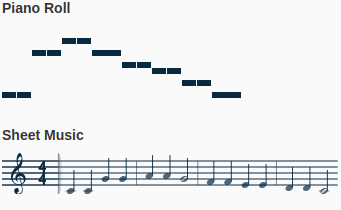
\includegraphics[width=0.5\textwidth]{../images/piano_roll.png}
    \caption{Esempio di rappresentazione di una partitura musicale in piano-roll}
\end{figure}

Il paper indicato, in particolare, presentava un implementazione delle metriche per l'estrazione di caratteristiche musicali basato su una rappresentazione delle partiture musicali in forma di \textbf{piano-roll}.
Il piano-roll è una rappresentazione grafica delle note musicali in cui l'asse delle ascisse rappresenta il tempo e l'asse delle ordinate rappresenta le note. Ogni cella della matrice corrisponde a una nota suonata in un determinato istante di tempo. Presenta tuttavia delle limitazioni, in quanto in condizioni particolari può esserci perdita di informazione.\
Invece che utilizzare il piano-roll, sono state estratte le caratteristiche direttamente dai file MIDI, quindi da una lista di note (\textbf{tuple}) con informazioni sul tempo, altezza, durata e strumento adoperato (nel nostro caso sempre e solo il clavicembalo), reimplementando le metriche del paper ma con questa diversa rappresentazione.\
Le caratteristiche estratte si dividono in due categorie: \textbf{caratteristiche ritmiche} e \textbf{caratteristiche tonali}. Le prime includono informazioni sul tempo e sulla durata delle note, mentre le seconde riguardano la tonalità delle note e le relazioni armoniche tra di esse.\
Tra le diverse distanze sono poi presenti: distanze scalari, distanze vettoriali e distanze matriciali.\

Le caratteristiche tonali considerate sono:
\begin{itemize}
    \item \textbf{number of pitches per measure} - il numero di toni diversi presenti in una singola battuta (vettore di dimensione 8)
    \item \textbf{pitch class histogram} - l'istogramma delle classi di toni presenti in una singola battuta (vettore di dimensione 12)
    \item \textbf{pitch class histogram per measure} - l'istogramma delle classi di toni presenti in una singola battuta (vettore di dimensione 12x8 = 96)
    \item \textbf{pitch class transition matrix} - la matrice di transizione delle classi di toni (matrice 12x12=144)
    \item \textbf{pitch range} - la differenza tra il tono più alto e il tono più basso (scalare)
    \item \textbf{average pitch shift} - la media delle variazioni di tono tra note consecutive (scalare)
\end{itemize}

Caratteristiche ritmiche:
\begin{itemize}
    \item \textbf{number of notes per measure} - il numero di note presenti in una singola battuta (vettore di dimensione 8)
    \item \textbf{note length histogram} - l'istogramma delle durata delle note presenti in una singola battuta (vettore di dimensione 24)
    \item \textbf{note length histogram per measure} - l'istogramma delle durata delle note presenti in una singola battuta (vettore di dimensione 24x8 = 192)
    \item \textbf{note length transition matrix} - la matrice di transizione delle durate delle note (matrice 24x24=576)
    \item \textbf{average IOI} - l'intervallo inter-onset medio, ovvero la media delle variazioni di durate di note consecutive (scalare)
\end{itemize}

Mentre per le immagini di farfalle avevamo un unico modello generativo per la generazione dei dati, per le partiture musicali sono stati utilizzati più modelli generativi, o meglio cinque versioni di uno stesso modello a diverse epoche di  \textit{training}.\

Il primo test eseguito è stato un \textbf{sanity check}, un controllo preliminare per garantire che le caratteristiche estratte mostrassero distribuzioni stabili e coerenti sui dati reali. 
Per fare ciò, sono state calcolate le KDE sulle distanze intra-set dei dati reali, suddivisi in \textbf{training} e \textbf{test} più \textbf{validation} set. Poiché entrambi i set contengono dati reali, una divergenza tra le distribuzioni, o una difficoltà
ad individuare una \textbf{bandwidth}, indicherebbe un problema nell’approccio o nelle caratteristiche selezionate.

Sono stati quindi riprodotti gli esperimenti condotti sul dataset di farfalle, studiando le distribuzioni delle distanze intra-set per ciascuna caratteristica sempre tramite KDE. Avendo a disposizione più modelli generativi sono stati prodotti grafici a violino (\textbf{violin plots}) che accostano le due distribuzioni e permettono di stabilire rapidamente quale epoca di training abbia prodotto i dati più simili a quelli reali.\
Per validare ulteriormente i risultati ottenuti, sono state tracciate le pr-curve (che seppur basate sulle distanze fra i dati, operano direttamente nello spazio dei dati e non sulle distanze).\

Sempre come nei test sul dataset di farfalle, sono stati identificati i falsi positivi individuando i dati generati che non rientravano nel manifold dei dati reali. In questa fase sono state anche calcolate le overlaped area tra le KDE dei dati reali e i dati genati dalle diverse epoche. 
Questo ha permesso di stabilire numericamente per ciascuna metrica quale epoca di training avesse prodotto i dati più simili a quelli reali per numero di falsi positivi e per overlaped area.\ 

Con 'measure' si intende una singola battuta di musica, ovvero un'unità di tempo musicale, ad esempio se il tempo è 4/4, una battuta è composta da 4 semiminime (o 8 crome, o 16 semicrome, ecc.).\
La maggior parte dei dati musicali di musica barocca è scritta in 4/4 con 8 battute, per quei dati in cui il tempo non era specificato è stato considerato 4/4, e in caso di battute mancanti sono state aggiunte battute vuote.\
Sebbene si sia cercato di eliminare i dati mal generati, alcuni di essi sono stati comunque inclusi nel dataset con le considerazioni sopra descritte. Ci aspettiamo che questo possa influenzare i risultati delle metriche, in particolare vogliamo verificare che l'applicazione delle metriche come filtro, siano in grado di discriminare tali dati di bassa qualità.\
Delle 1000 partiture musicali per modello disponibili ne sono state scartate le prime 50 e le ultime 50, per un totale di 900 partiture musicali per modello.\
Gli altri iperparametri e distanze utilizzate sono state le stesse di quelle impiegate per il dataset di farfalle, fatta eccezione del valore di \texttt{k} che è stato impostato a \texttt{k = 3} per tutte le metriche. La motivazione è che ci aspettiamo che i dati musicali siano più fitti di quelli delle immagini (sopratutto date le caratteristiche estratte) e quindi un valore di \texttt{k} più basso dovrebbe permettere una stima del manifold più accurata.\

Infine, sempre per studiare le capacità delle metriche di discriminare dati di alta e bassa qualità, è stato adottato un approccio \textbf{leave-one-out} applicato però alla stima della KDE.\
È stato rimosso dalla KDE stimata dalle distanze inter-set fra dati reali e dati generati da una certa epoca, i contributi di ciascun dato generato e verificato se la \textbf{likelihood} di tale dato fosse inferiore ad un certo \textbf{threshold}.
Nel caso in cui la likelihood fosse inferiore al threshold il dato generato è da considerare un falso positivo.\
Come trashold è stato preso lo \texttt{0.05} percentile delle likelihood stimate con la KDE.\
Questo metodo, sebbene efficace, ha un enorme limitazione, infatti prendendo un percentile fisso avremo lo stesso numero di falsi positivi per ogni epoca di training, questo non ci permette di confrontare le epoche tra di loro, ma solo di valutare la capacità delle metriche di discriminare dati di alta e bassa qualità.\
Metodi più sofisticati prevedono di calcolare la GPD (Generalized Pareto Distribution) sulle likelihood stimate e prendere il threshold in modo da identificare con maggiore accuratezza l'insieme completo degli outliers, vedi \cite{9LeaveOneOut}, ma questo è stato considerato fuori dallo scopo di questo lavoro.